\documentclass[12pt] {article}
\usepackage{enumerate}
\usepackage{algorithm2e}
\usepackage{mcode}
\usepackage{listings}
\usepackage{graphicx}
\usepackage{epsf}

\author{Zhengwu Zhang}
\title{Homework 2}

\begin{document} 
\maketitle
 
\newpage
Problem 1. \\
a) \\
 (i) $X_t$ is irreducible, because every elements in the transition matrix $\Pi$ is big than 0. \\
 (ii) Since $d(x_1)=1$, $d(x_2)=1$, $d(x_3)=1$, $d(x_4)=1$, this irreducible Markov Chain is aperiodic. \\
 (iii) The stationary probability vector $X_t=$[0.5 0.5 0.5 0.5], matlab code:
  \begin{lstlisting}
% for homework 2
% problem 1

clear; close all;

PI = [0.1 0.3 0.4 0.2; 0.2 0.1 0.3 0.4; 0.4 0.2 0.1 0.3; 0.3 0.4 0.2 0.1];  % transition matrix

[V, D] = eig(PI'); 
ind = find(abs(diag(D)-1)< 1e-6);
P = V(:,ind)/sum(V(:,ind));
  \end{lstlisting}

b)\\
\begin{figure}
\begin{center}

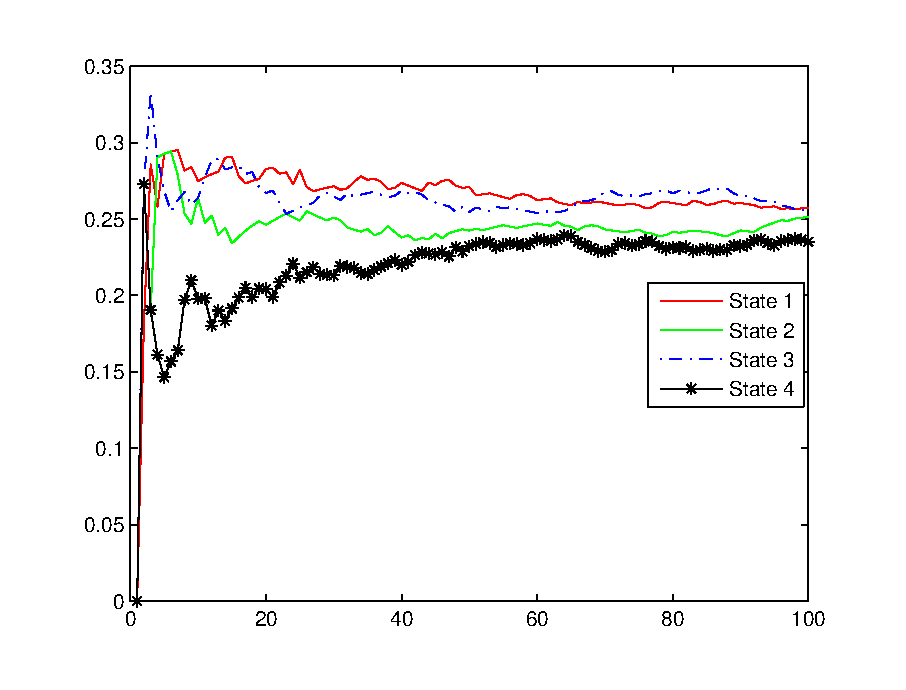
\includegraphics[height=2.2 in] {hm2_prob1_b.eps}
\caption{Averages along one path converge to the stationary probability}

\end{center}
\end{figure}

\begin{lstlisting}
% for homework 2
% problem 1

clear; close all;

PI = [0.1 0.3 0.4 0.2; 0.2 0.1 0.3 0.4; 0.4 0.2 0.1 0.3; 0.3 0.4 0.2 0.1];  % transition matrix

M = 4;      % number of chains
N = 4;      % number of states
K = 1000;    % number of time steps in each chain

for m = 1:M
    %x(1,m) = m;  % random initial
     x(1,m) = ceil(4*rand);
    for k = 2:K
        % generate a chain
        P = PI(x(k-1,m),:); %pick i-th row
        U = rand;
        if U < P(1)
            x(k,m) = 1;
            
        elseif (P(1)<U&&U<(P(1)+P(2)))
            x(k,m) = 2;
            
        elseif((P(1)+P(2))<U&&U<(P(1)+P(2)+P(3)))
                    
                    x(k,m) = 3;
        else
            x(k,m) = N; 
        end
        for n=1:N
        p0(m,n,k) = sum(x(:,m)==n)/k;
        end;
    end
end

plot(squeeze(p0(1,1,1:10:1000)),'r');
hold on,plot(squeeze(p0(1,2,1:10:1000)),'-g');
hold on,plot(squeeze(p0(1,3,1:10:1000)),'-.b');
hold on,plot(squeeze(p0(1,4,1:10:1000)),'-*k');

\end{lstlisting}

c)\\
\begin{figure}
\begin{center}
\includegraphics[height=2.2 in] {hm2_prob1_c.eps}
\caption{Simulation}
\end{center}
\end{figure}

\begin{lstlisting}
% for homework 2
% problem 1

clear; close all;

PI = [0.1 0.3 0.4 0.2; 0.2 0.1 0.3 0.4; 0.4 0.2 0.1 0.3; 0.3 0.4 0.2 0.1];  % transition matrix

f=[2.0 1.0 2.5 -1.0];

N=4; % state #
K=1000;

%generate the chain
 x(1,1) = ceil(4*rand);
    for k = 2:K
        % generate a chain
        P = PI(x(k-1,1),:); %pick i-th row
        U = rand;
        if U < P(1)
            x(k,1) = 1;
            
        elseif (P(1)<U&&U<(P(1)+P(2)))
            x(k,1) = 2;
            
        elseif((P(1)+P(2))<U&&U<(P(1)+P(2)+P(3)))
                    
                    x(k,1) = 3;
        else
            x(k,1) = N; 
        end
    end
 
[V, D] = eig(PI'); 
ind = find(abs(diag(D)-1)< 1e-6);
P = V(:,ind)/sum(V(:,ind));
    
% generate the estimator

for i=1:10:1000
Est1(i)=(1/i)*sum(f(x(1:i,1)));
Est2(i)=sum(f*P);
end;

plot(Est1(1:10:1000),'r');
hold on, plot(Est2(1:10:1000),'--b')
\end{lstlisting}


Problem 2 \\
a) \\
\begin{lstlisting}

>> PI = [0.1 0.3 0.4 0.2; 0.2 0.4 0 0.4; 0 0.3 0.5 0.2; 0.5 0.3 0.2 0]; 
>> PI*PI

ans =

    0.1700    0.3300    0.2800    0.2200
    0.3000    0.3400    0.1600    0.2000
    0.1600    0.3300    0.2900    0.2200
    0.1100    0.3300    0.3000    0.2600
\end{lstlisting}

So the elements in $\Pi^2$ is all big than 0, $X_t$ is irreducible.  Since $d(x_1)=1$, $d(x_2)=1$, $d(x_3)=1$, $d(x_4)=1$, $X_t$ is aperiodic. 
$P =$[0.1975    0.3333    0.2469    0.2222]

b) \\ 
See figure 3.

\begin{figure}
\begin{center}
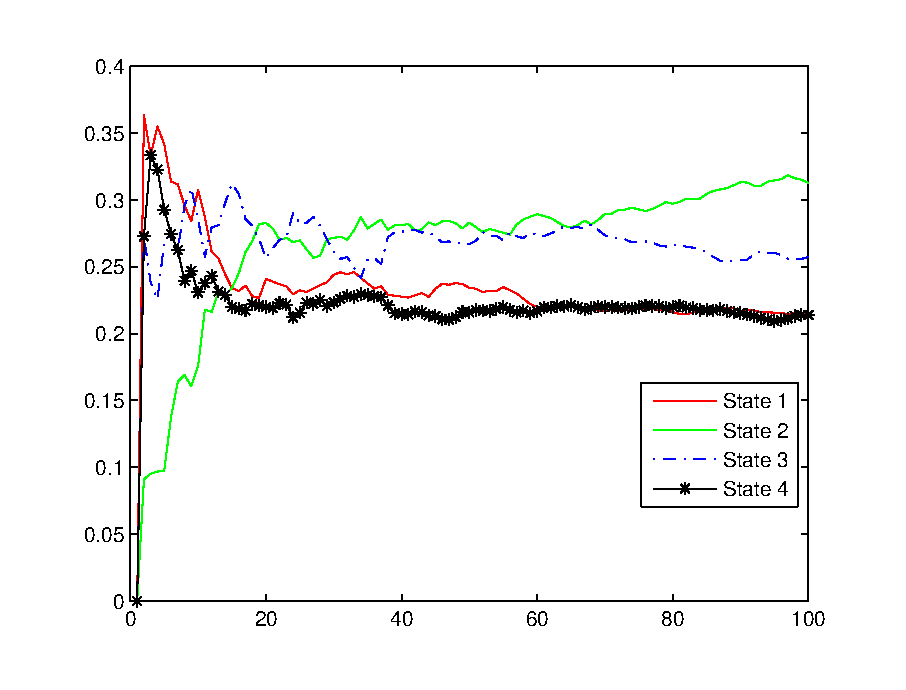
\includegraphics[height=2.2 in] {hm2_prob2_b.eps}
\caption{Averages along one path converge to the stationary probability}
\end{center}
\end{figure}

c)\\
See figure 4

\begin{figure}
\begin{center}
\includegraphics[height=2.2 in] {hm2_prob2_c.eps}
\caption{Simulation}
\end{center}
\end{figure}

\end{document}